\documentclass{article}
\usepackage{tikz}

\begin{document}
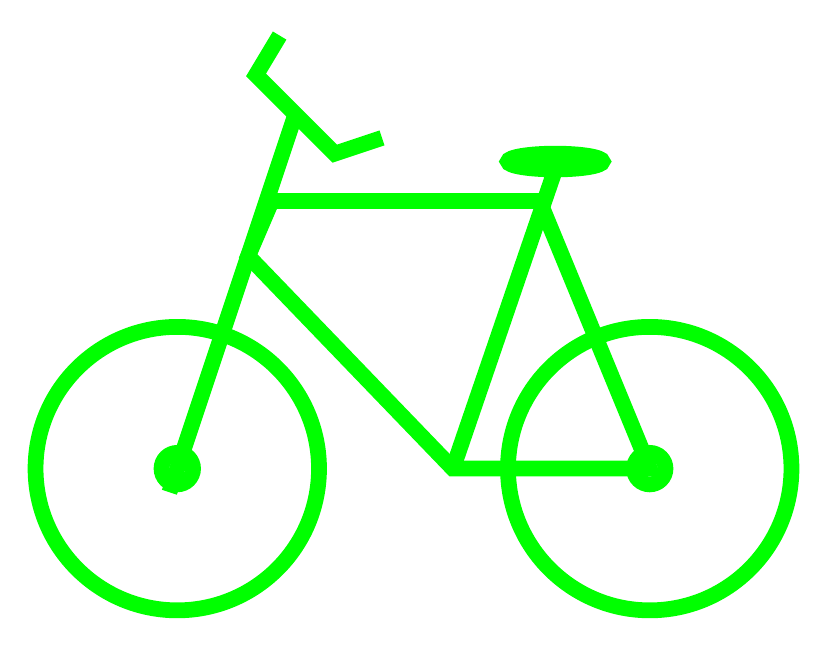
\begin{tikzpicture}[color=green,line width=2mm]

%front and back wheels
\draw (10,3) circle(1.8); \draw (10,3) circle(0.2);
\draw (4,3) circle(1.8);  \draw (4,3) circle(0.2);

%central bracket (polygon with 5 sides)
\draw (10,3) -- (8.6,6.4) -- (5.2,6.4) -- (4.9,5.7)
-- (7.5,3) --cycle;

%handle and seat rods
\draw (3.9,2.7) -- (5.5,7.5); \draw (7.5,3) -- (8.8,6.8);

%handle and seat
\draw (5.3,8.5) -- (5,8) -- (6,7) -- (6.6,7.2);
\draw (8.8,6.9) ellipse (0.6 and 0.1);
\end{tikzpicture}
\end{document}